\documentclass[aspectratio=169, 10pt]{beamer}

% --- Pacchetti Principali ---
\usepackage[utf8]{inputenc}
\usepackage{amsmath, amssymb, amsfonts, bm}
\usepackage{mathtools}
\usepackage{booktabs}
\usepackage{graphicx}
\usepackage{hyperref}
\usepackage{microtype}
\usepackage{tikz}

% --- Tema e Stile ---
\usetheme{Madrid}
\usecolortheme{seahorse}

\setbeamertemplate{navigation symbols}{}
\setbeamertemplate{caption}[numbered]

% Palette colori personalizzata
\definecolor{primaryColor}{RGB}{24, 43, 73}
\definecolor{secondaryColor}{RGB}{41, 128, 185}
\definecolor{accentColor}{RGB}{231, 76, 60}

\setbeamercolor{structure}{fg=secondaryColor}
\setbeamercolor{palette primary}{bg=primaryColor,fg=white}
\setbeamercolor{palette secondary}{bg=secondaryColor,fg=white}
\setbeamercolor{palette tertiary}{bg=primaryColor!90,fg=white}
\setbeamercolor{titlelike}{parent=palette primary}
\setbeamercolor{block title}{bg=primaryColor!10,fg=primaryColor}
\setbeamercolor{block body}{bg=primaryColor!5,fg=black}

% --- Metadati Presentazione ---
\title[Iron Stats]{Ottimizzazione Numerica e Biomeccanica Funzionale dell'Allenamento}
\subtitle{Modellazione Funzionale, Metriche Dinamiche e Simulated Annealing}
\author{Lorenzo Zambardi}
\date{A.A. 2025-2026}

\begin{document}

% -------------------------------------------------------------
% SLIDE TITOLO & INDICE
% -------------------------------------------------------------
\begin{frame}
    \titlepage
\end{frame}

\begin{frame}{Indice}
    \tableofcontents
\end{frame}

% =============================================================
\section{1. Introduzione e Motivazione}
% =============================================================

\begin{frame}{1.1 Limiti dei Modelli Discreti Tradizionali}
    \begin{itemize}
        \item \textbf{Approccio Scalare Classico:}
        \begin{itemize}
            \item $\text{Volume} = \text{Serie} \times \text{Ripetizioni}$
            \item $\text{Tonnellaggio grezzo} = \text{Serie} \times \text{Reps} \times \text{Carico}$
        \end{itemize}
        \vspace{0.3cm}
        \item \textbf{Criticità Fisiologiche e Meccaniche:}
        \begin{itemize}
            \item Incapacità di modellare la variazione continua del \textbf{braccio di leva} muscolo-articolare.
            \item Ignora il \textbf{profilo di resistenza} delle macchine o dei pesi liberi lungo il Range of Motion (ROM).
            \item Mancata stima dell'\textbf{affaticamento neuromuscolare intrinseco} e della caduta di velocità concentrica.
        \end{itemize}
    \end{itemize}
\end{frame}

\begin{frame}{1.2 Formulazione del Problema Numerico}
    \begin{block}{Transizione al Continuo}
        Si passa da variabili scalari a \textbf{campi funzionali continui} parametrizzati sull'angolo o quota di escursione articolare:
        $$t \in [0, 1] \quad (\text{Range of Motion - ROM})$$
    \end{block}
    \vspace{0.2cm}
        L'ottimizzazione del programma settimanale viene formulata come un \textbf{Problema di minimo globale multiobiettivo vincolato su spazio discreto combinatorio}
\end{frame}

\begin{frame}{1.3 Obiettivi di Calcolo Scientifico e Metodi Numerici}
    \begin{columns}[T]
        \begin{column}{0.48\textwidth}
            \begin{block}{Approssimazione Funzionale}
                Studio comparativo di accuratezza, stabilità e condizionamento numerico:
                \begin{itemize}
                    \item Interpolazione di Lagrange/Newton
                    \item Spline Cubiche ($C^2$)
                    \item Curve Parametriche di Bézier (Bernstein)
                \end{itemize}
            \end{block}
        \end{column}
        \begin{column}{0.48\textwidth}
            \begin{block}{Quadratura \& Ottimizzazione}
                \begin{itemize}
                    \item Conservazione rigorosa della magnitudo tramite \textbf{formula composita dei trapezi}.
                    \item Adimensionalizzazione dei gradienti d'errore via simulazione \textbf{Monte Carlo}.
                    \item Euristica di convergenza globale: \textbf{Simulated Annealing}.
                \end{itemize}
            \end{block}
        \end{column}
    \end{columns}
\end{frame}

% =============================================================
\section{2. Models: Modellazione e Approssimazione Funzionale}
% =============================================================

\begin{frame}{2.1 Formalizzazione della Classe Esercizio}
    \begin{block}{Parametri Biomeccanici}
        \begin{itemize}
            \item $c_{load} \in (0, 1]$: Efficienza articolare e dispersione del carico.
            \item $f_{base} \in [1, 10]$: Coefficiente intrinseco di affaticamento sistemico.
            \item $\mu_{load} \in \mathbb{R}^+, \; q_{load} \in \mathbb{R}$: Correzione carico effettivo: $L = L_{nom} \cdot \mu_{load} + q_{load}$.
            \item $is\_isolation \in \{0, 1\}$: Flag booleano esercizio mono/multi-articolare.
        \end{itemize}
    \end{block}
    \begin{alertblock}{Vincolo di Conservazione della Ripartizione Muscolare}
        Per l'insieme dei distretti $\mathcal{M}$ e vettore magnitudo $\mathbf{M} = [M_1, \dots, M_k]^T$:
        $$\sum_{m \in \mathcal{M}} M_m = 1.0 \pm \varepsilon, \quad \varepsilon \le 10^{-4}$$
        \footnotesize \textbf{Tolleranza numerica $\varepsilon$:} dovuta all'aritmetica floating-point IEEE 754 e all'arrotondamento delle percentuali nei file di configurazione JSON ($M_m = \text{pct} / 100$).
    \end{alertblock}
\end{frame}

\begin{frame}{2.2 Analisi Numerica: Interpolazione di Lagrange e Runge (1/3)}
    \begin{columns}[T]
        \begin{column}{0.48\textwidth}
            \begin{block}{Interpolazione Polinomiale Globale}
                Dati $n$ nodi equispaziati su $t \in [0, 1]$:
                $$p_{n-1}(t) = \sum_{i=1}^n y_i \ell_i(t)$$
            \end{block}
            \begin{alertblock}{Instabilità Numerica e Runge}
                \begin{itemize}
                    \item \textbf{Vandermonde:} condizionamento divergente esponenzialmente ($\kappa(V) \gg 10^6$).
                    \item \textbf{Fenomeno di Runge:} oscillazioni parassite ai bordi del ROM:
                    $$\lim_{n \to \infty} \max_{t \in [0, 1]} |f(t) - p_n(t)| = \infty$$
                    \item Genera forze e tensioni fittizie non fisiche.
                \end{itemize}
            \end{alertblock}
        \end{column}
        \begin{column}{0.50\textwidth}
            \centering
            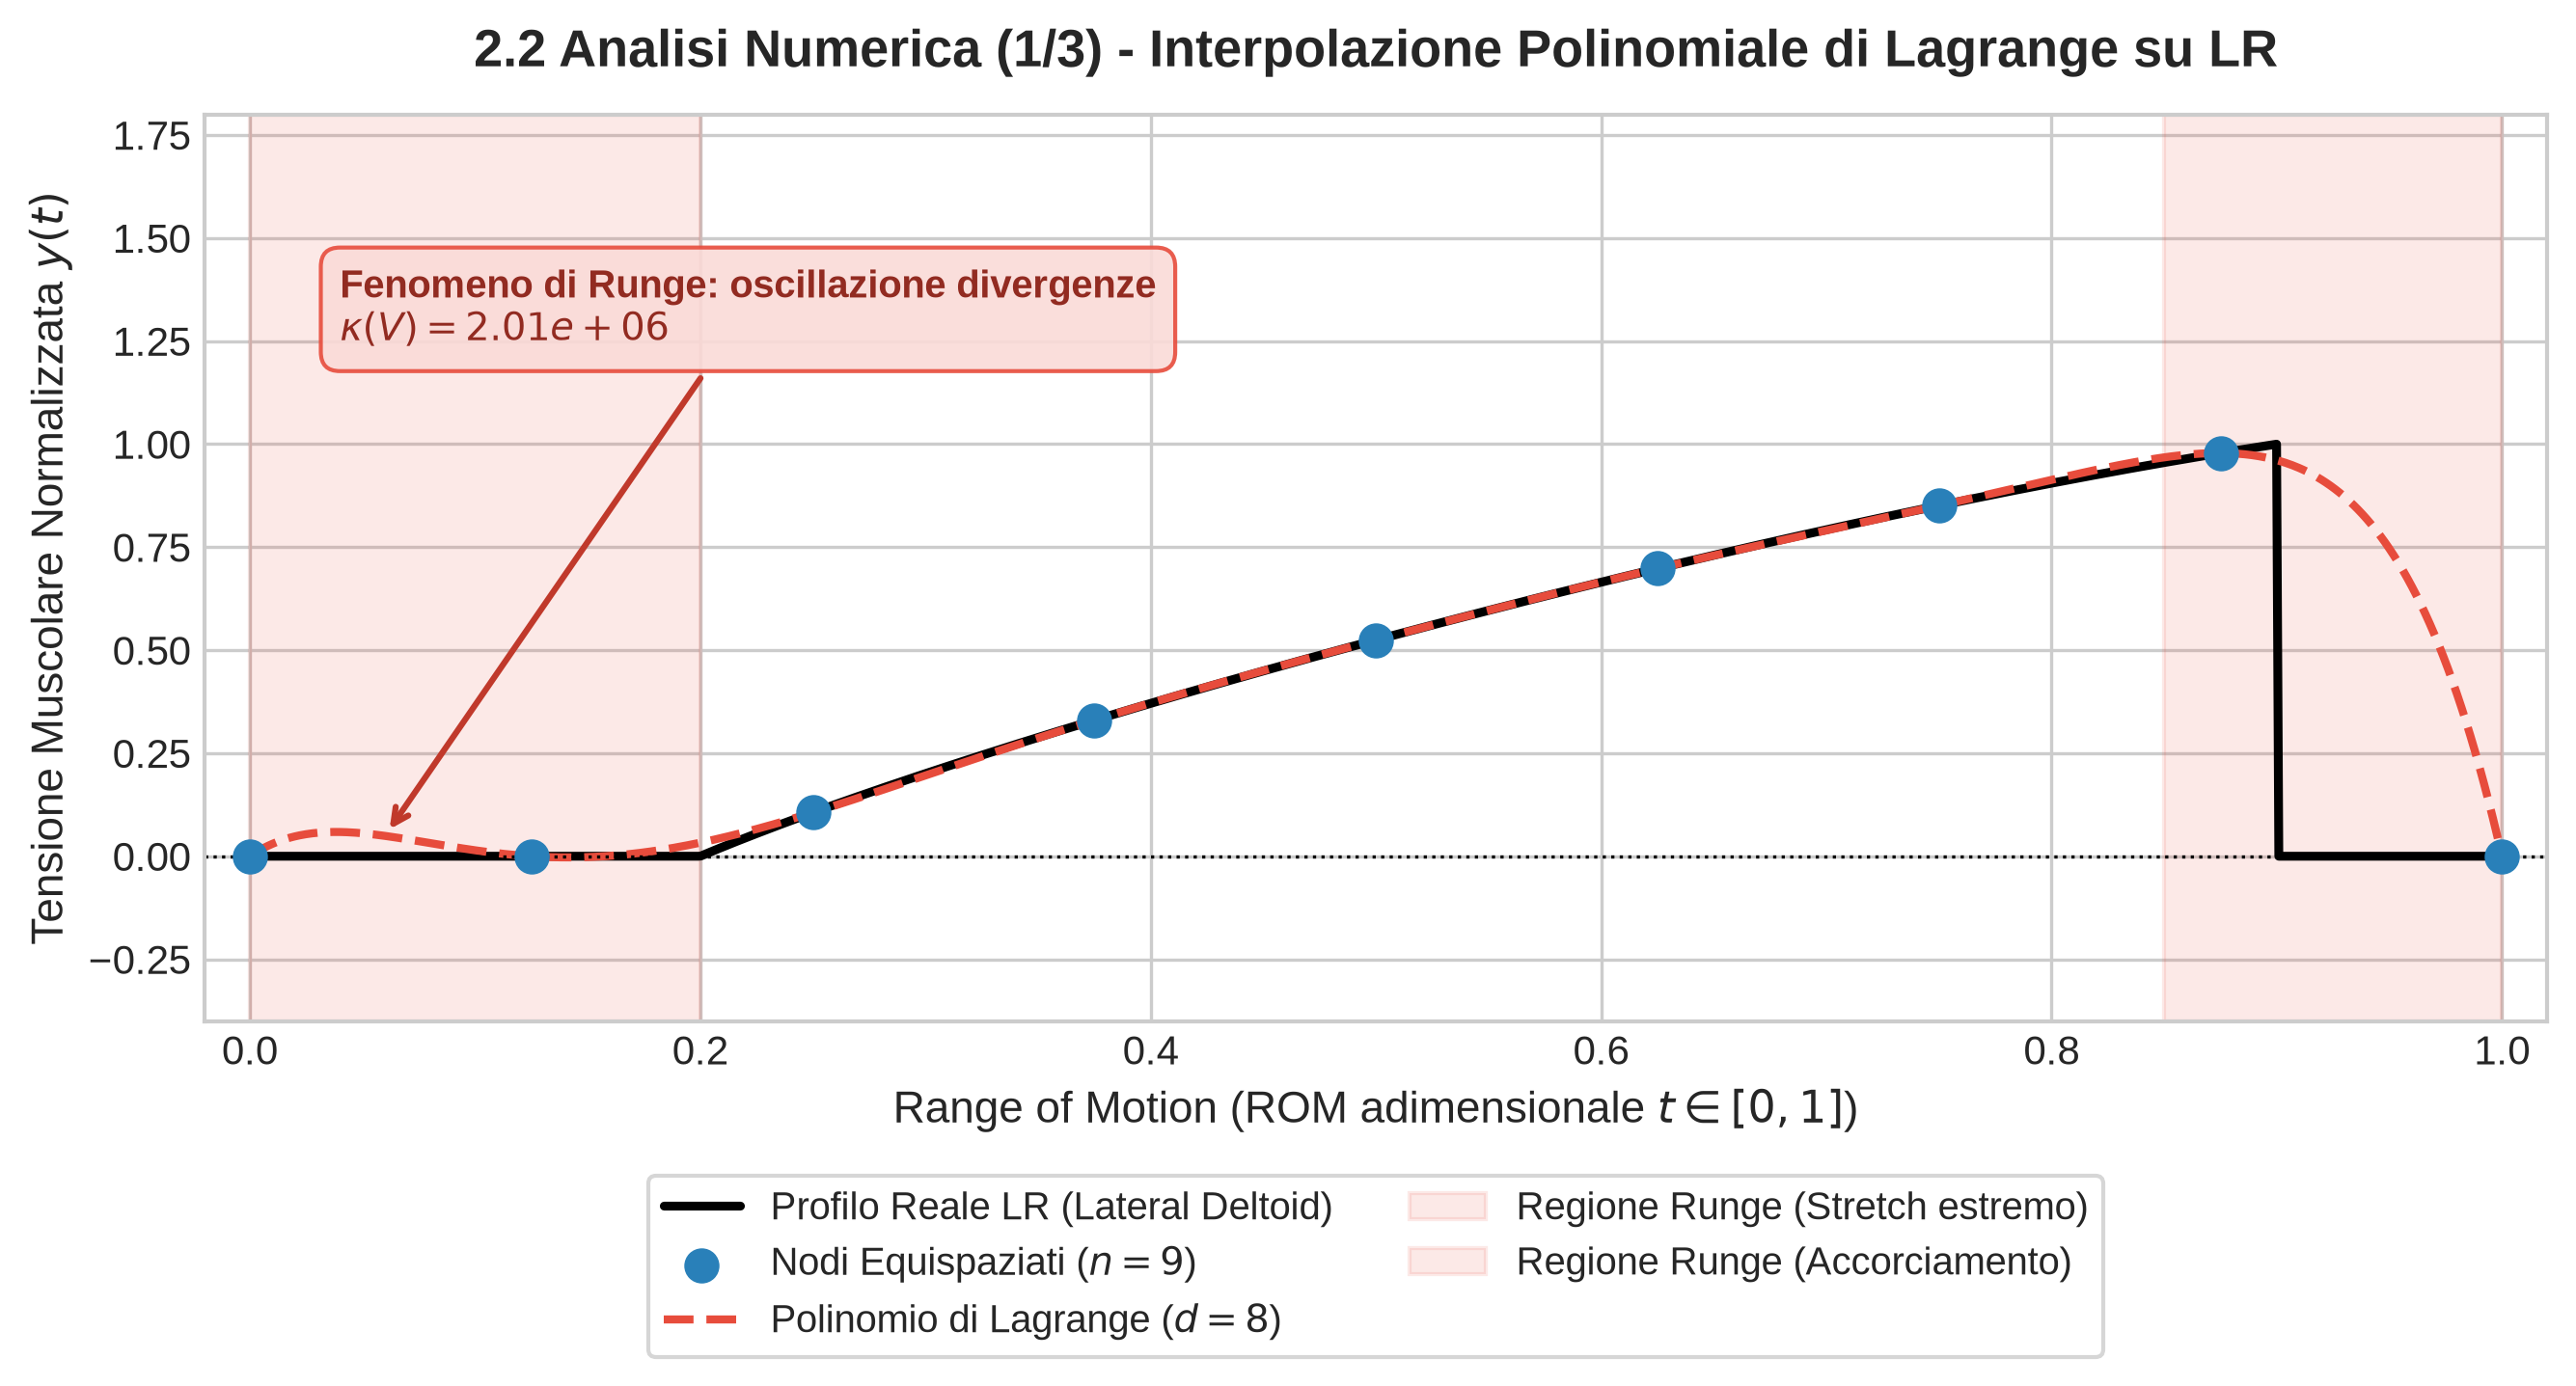
\includegraphics[width=\linewidth]{plot_lagrange_runge.png}
            \scriptsize \textbf{Caso studio LR (Lateral Raise):} con $n=9$ nodi equispaziati, l'interpolante diverge drasticamente agli estremi di allungamento ($t \to 0$) e accorciamento ($t \to 1$).
        \end{column}
    \end{columns}
\end{frame}

\begin{frame}{2.2 Analisi Numerica: Spline Cubiche e Undershoot (2/3)}
    \begin{columns}[T]
        \begin{column}{0.48\textwidth}
            \begin{block}{Proprietà delle Spline Cubiche}
                Raccordo a tratti con continuità $C^2$:
                \begin{itemize}
                    \item Sistema tridiagonale $A \mathbf{m} = \mathbf{d}$ in tempo lineare $\mathcal{O}(n)$ via \textbf{Algoritmo di Thomas}.
                    \item Risolve le oscillazioni globali di Runge.
                \end{itemize}
            \end{block}
            \begin{alertblock}{Violazione dei Vincoli Fisici}
                \begin{itemize}
                    \item \textbf{Overshoot e Undershoot:} assenza del vincolo di monotonicità/positività:
                    $$y(t) < 0$$
                    \item \textbf{Inconsistenza fisica:} un muscolo non può erogare tensione contrattile attiva negativa.
                \end{itemize}
            \end{alertblock}
        \end{column}
        \begin{column}{0.50\textwidth}
            \centering
            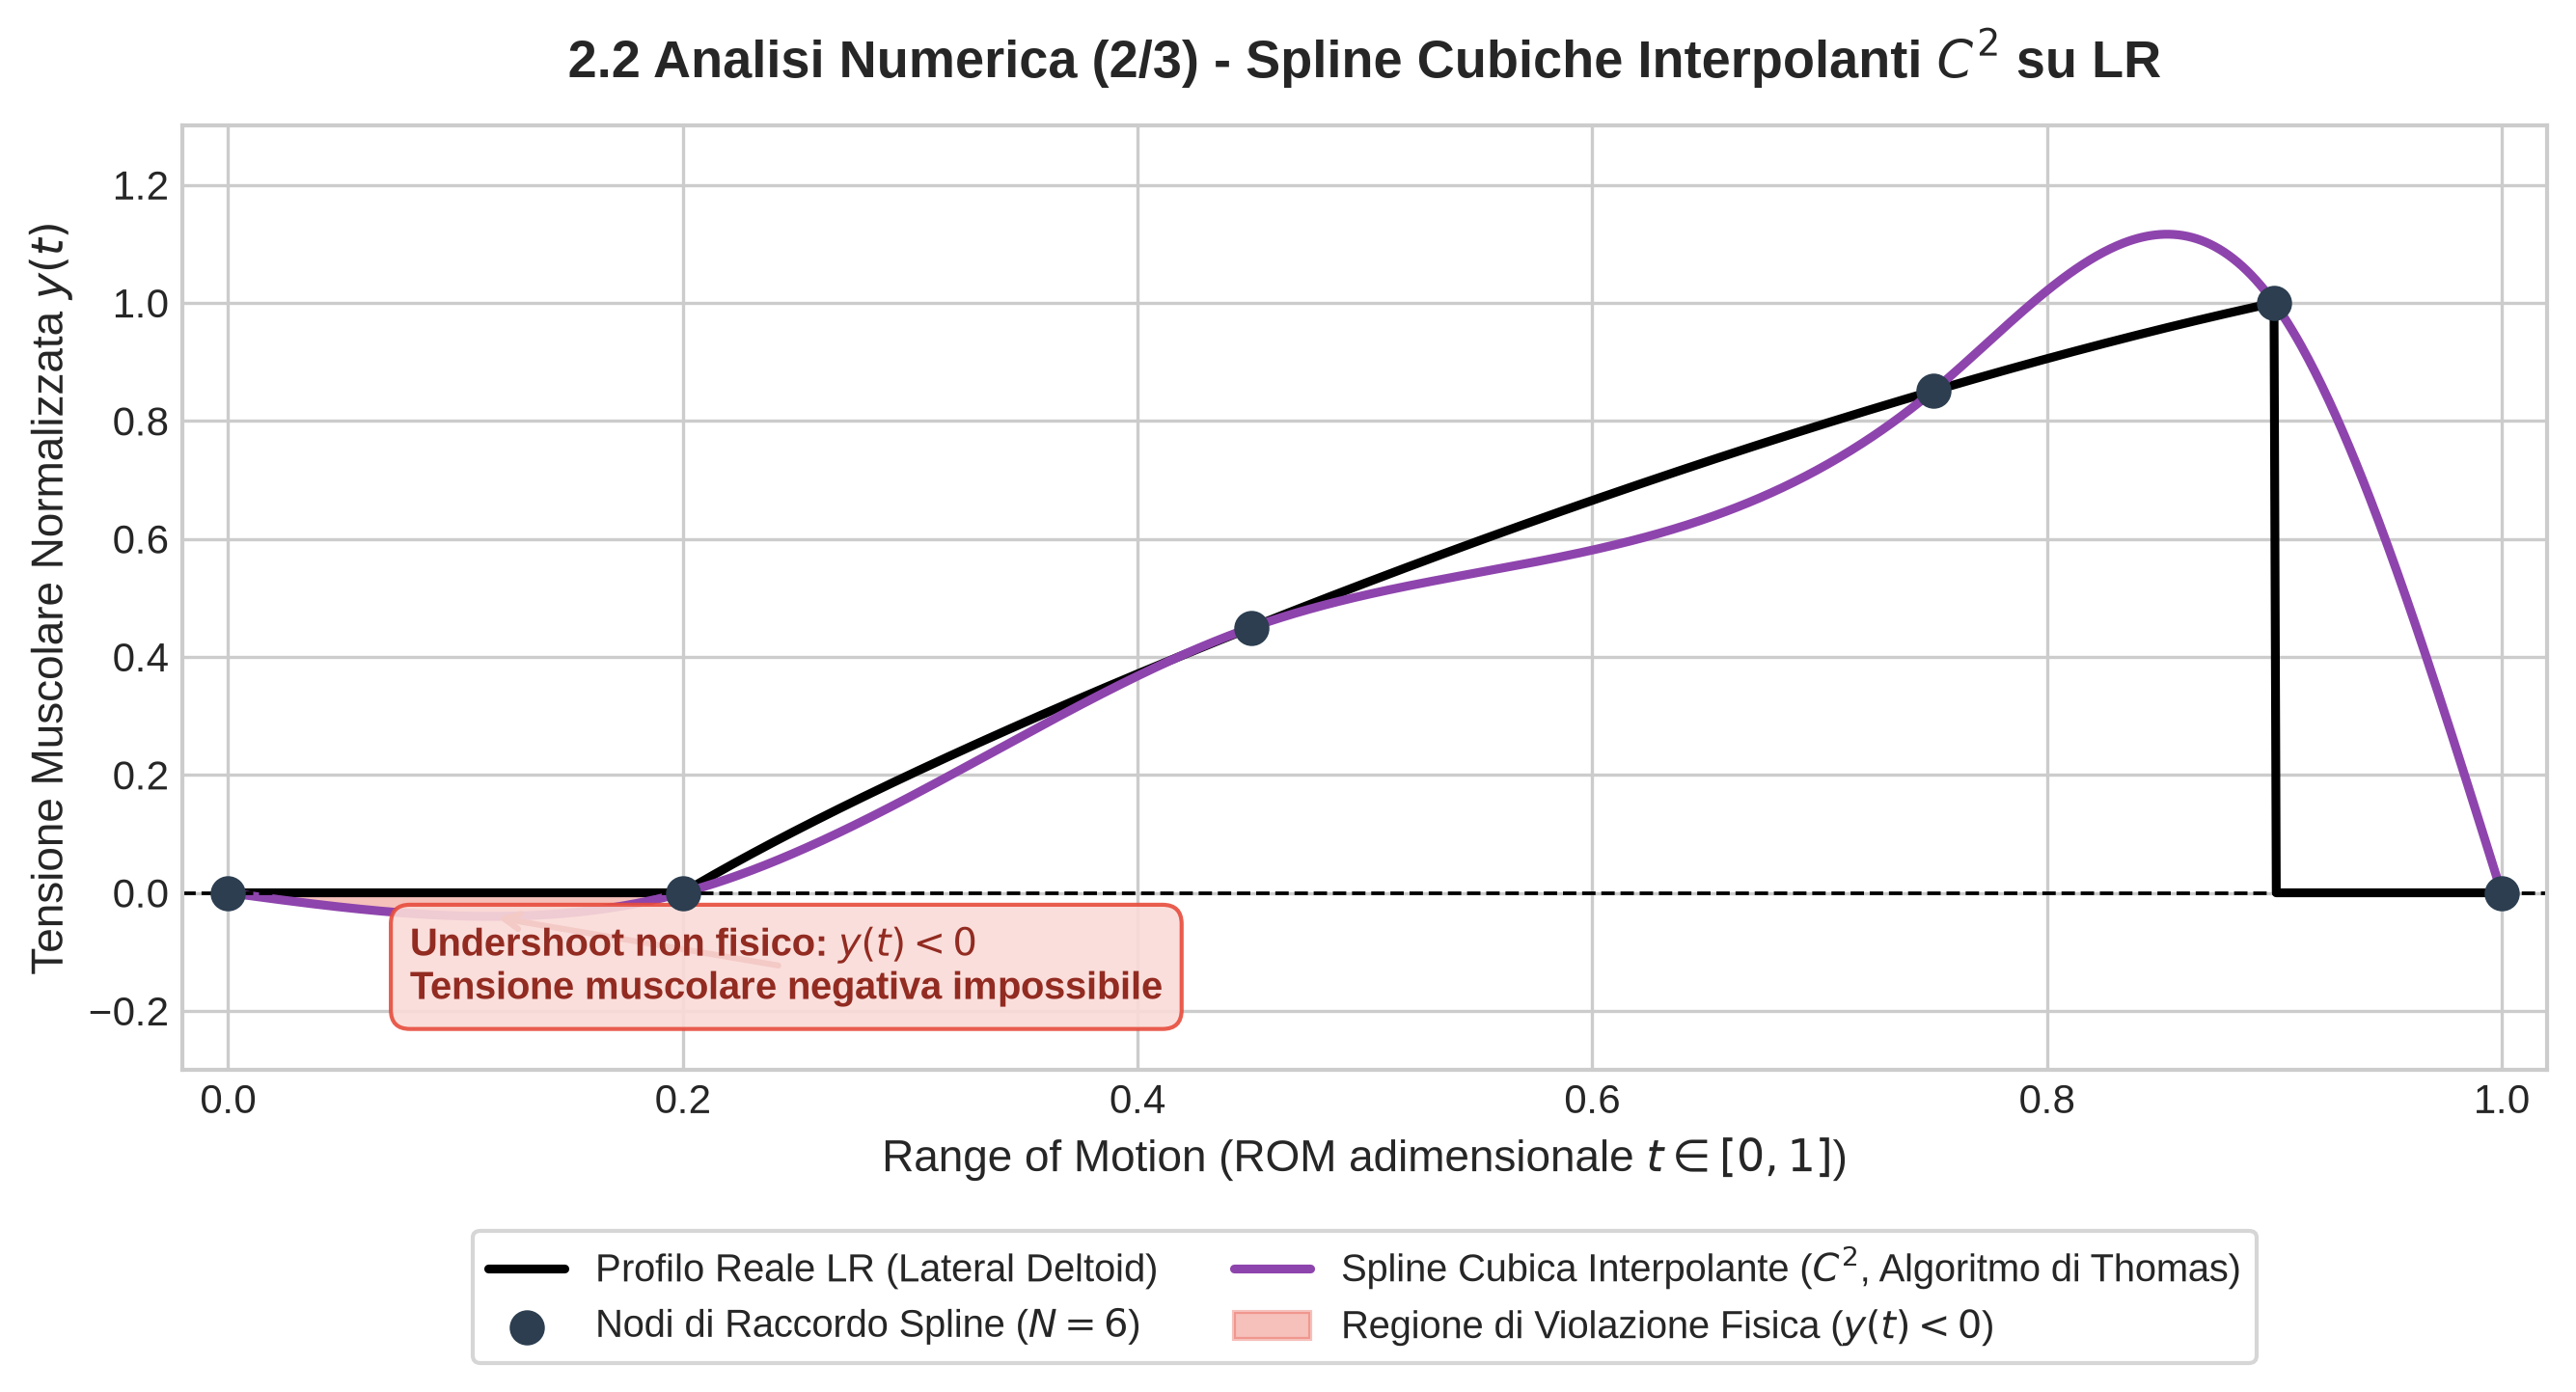
\includegraphics[width=\linewidth]{plot_spline_overshoot.png}
            \scriptsize \textbf{Caso studio LR (Lateral Raise):} la spline naturale produce un marcato undershoot ($y(t) < 0$) in fase di allungamento iniziale ($t \in [0, 0.2]$).
        \end{column}
    \end{columns}
\end{frame}

\begin{frame}{2.2 Analisi Numerica: Curve di Bézier e Confronto (3/3)}
    \begin{columns}[T]
        \begin{column}{0.48\textwidth}
            \begin{block}{Polinomi di Bernstein di Grado 3}
                $$\mathbf{P}(t) = \sum_{i=0}^3 \mathbf{P}_i B_{i,3}(t), \quad B_{i,3}(t) = \binom{3}{i} t^i (1-t)^{3-i}$$
            \end{block}
            \begin{block}{Garanzie Matematiche e Numeriche}
                \begin{itemize}
                    \item \textbf{Partizione dell'Unità:} $\sum_{i=0}^3 B_{i,3}(t) \equiv 1$.
                    \item \textbf{Inviluppo Convesso (Convex Hull):}
                    \begin{align*}
                    B_{i,3}(t) \ge 0 &\implies \mathbf{P}(t) \in \text{Conv}(\{\mathbf{P}_i\}) \\
                    &\implies y(t) \ge 0 \quad \forall t \in [0, 1]
                    \end{align*}
                    \item \textbf{Complessità $\mathcal{O}(1)$:} forma analitica o De Casteljau.
                \end{itemize}
            \end{block}
        \end{column}
        \begin{column}{0.50\textwidth}
            \centering
            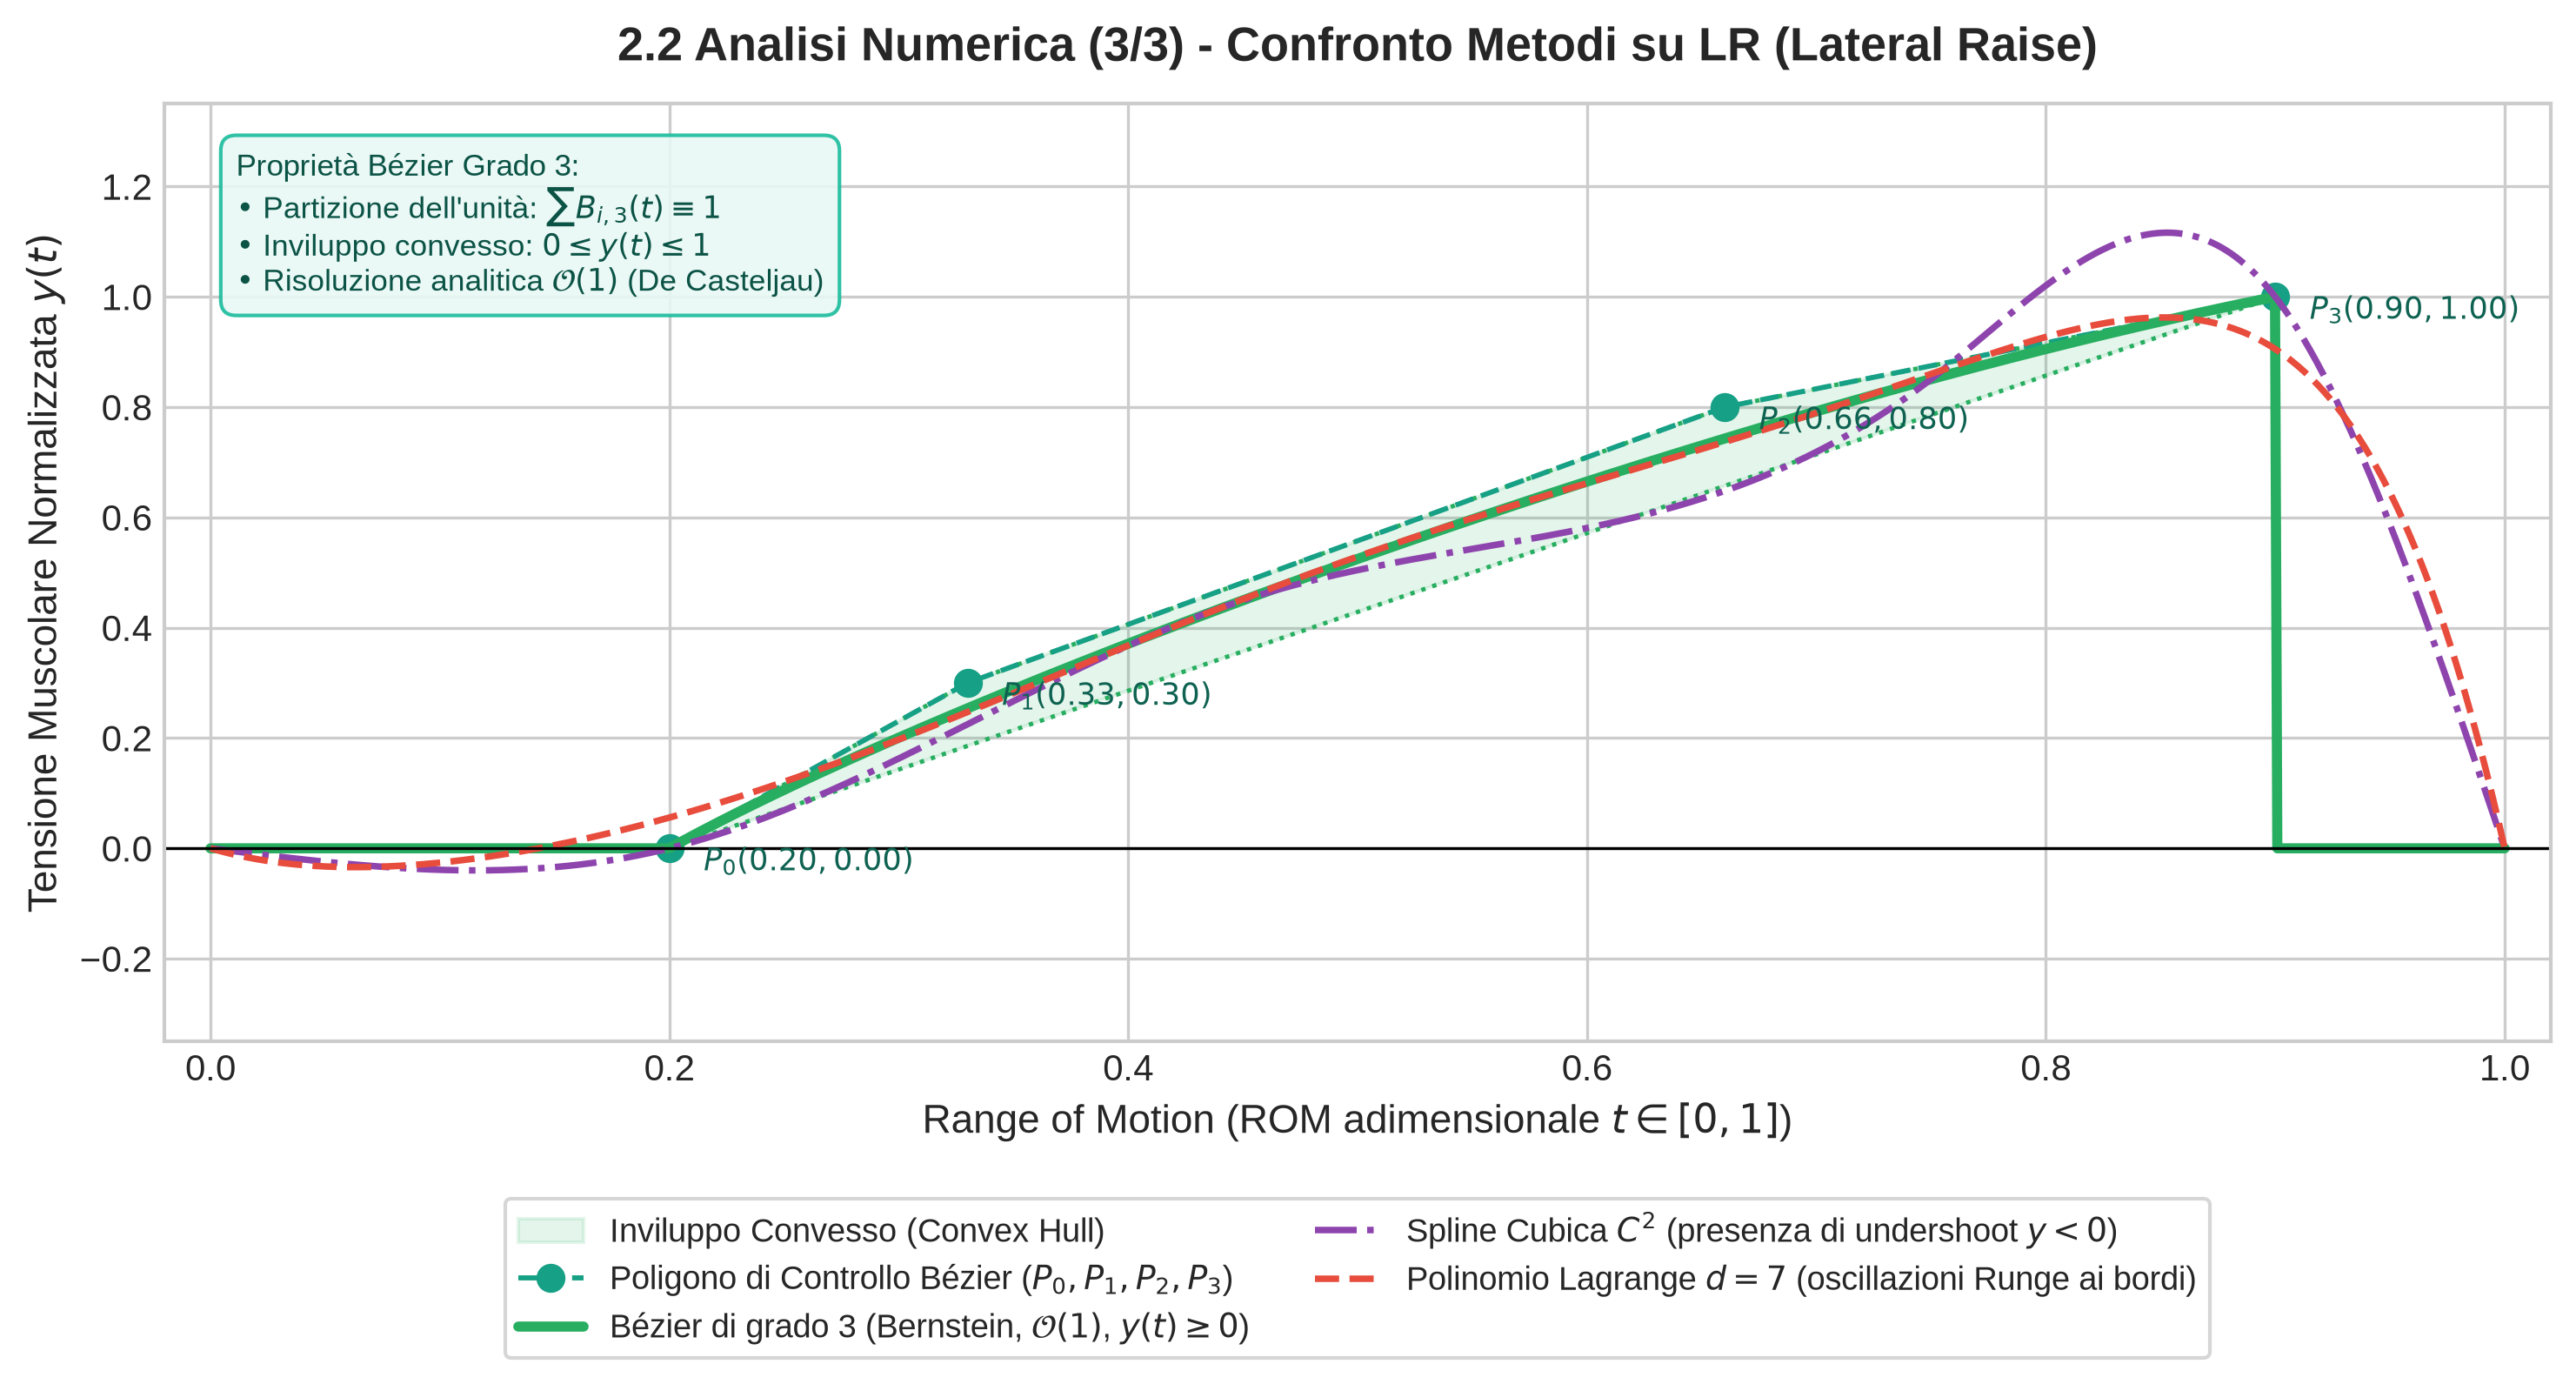
\includegraphics[width=\linewidth]{plot_bezier_confronto.png}
            \scriptsize \textbf{Sintesi Comparativa su LR:} Bézier (in verde) rispetta rigorosamente il poligono di controllo $\{P_0, \dots, P_3\}$, priva di oscillazioni o valori negativi.
        \end{column}
    \end{columns}
\end{frame}

\begin{frame}{2.3 Quadratura Numerica e Riscalamento Vincolato}
    \begin{block}{Calcolo dell'Area Sotto la Curva (AUC)}
        Griglia discreta $N = 50$, passo $h = \Delta t = \frac{1}{N-1}$:
        $$I_{trap} = \int_0^1 y(x)\,dx \approx \sum_{k=0}^{N-2} \frac{y(t_k) + y(t_{k+1})}{2} (t_{k+1} - t_k)$$
        Errore di troncamento della formula composita: $E_{trap} = -\frac{1}{12(N-1)^2} y''(\xi) = \mathcal{O}(h^2)$.
    \end{block}
    \begin{block}{Operatore di Riscalamento Funzionale}
        Garantisce che l'integrale coincida esattamente con la magnitudo target $M$:
        $$\tilde{y}(t) = \begin{cases} y(t) \cdot \frac{M}{I_{trap}} & \text{se } I_{trap} > 0 \\ \mathbf{0} & \text{altrimenti} \end{cases} \implies \int_0^1 \tilde{y}(t)\,dt = M + \mathcal{O}(h^2)$$
    \end{block}
\end{frame}

% =============================================================
\section{3. Analizzatore: Dinamica Discreta e Metriche di Carico}
% =============================================================

\begin{frame}{3.1 Volume ($V$) ed Effective Volume ($V_{eff}$)}
    \begin{itemize}
        \item \textbf{Ripetizioni Totali Equivalenti (serie $s$):}
        $$R_{tot, s} = R_{base, s} + c_{ass} R_{ass, s} + c_{part} R_{part, s} \quad (c_{ass}=0.5, \, c_{part}=0.33)$$
        \item \textbf{Ripetizioni Efficaci da Scala RPE ($RPE \in [0, 10]$):}
        $$R_{eff, s} = \min\Big(R_{base, s}, \, \max\big(0, \, RPE_s - 4.0\big)\Big) + c_{ass} R_{ass, s} + c_{part} R_{part, s}$$
        \item \textbf{Proiezione sulla quota muscolare $\Omega_m = \int \tilde{y}_m(t) dt$:}
        $$V = \sum_{s} R_{tot, s} \cdot \Omega_m, \qquad V_{eff} = \sum_{s} R_{eff, s} \cdot \Omega_m$$
    \end{itemize}
\end{frame}

\begin{frame}{3.2-3.3 Tonnellaggio e Tonnellaggio Ponderato}
    \begin{columns}[T]
        \begin{column}{0.48\textwidth}
            \begin{block}{Tonnellaggio ($T$ e $T_{eff}$)}
                Carico effettivo: $L_s = L_{nom, s} \cdot \mu_{load} + q_{load}$.
                $$T = \sum_{s} (L_s \cdot R_{tot, s}) \cdot \Omega_m$$
                $$T_{eff} = \sum_{s} (L_s \cdot R_{eff, s}) \cdot \Omega_m$$
            \end{block}
        \end{column}
        \begin{column}{0.48\textwidth}
            \begin{block}{Tonnellaggio Ponderato ($T_w, T_{w,eff}$)}
                Include l'efficienza articolare $c_{load}$:
                $$T_w = \sum_{s} (L_s R_{tot, s} c_{load}) \Omega_m$$
                $$T_{w,eff} = \sum_{s} (L_s R_{eff, s} c_{load}) \Omega_m$$
            \end{block}
        \end{column}
    \end{columns}
\end{frame}

\begin{frame}{3.4 TUT (Time Under Tension) e Decadimento di Velocità}
    \begin{itemize}
        \item Tempo base per ripetizione: $\tau_0 = t_{conc} + t_{iso,short} + t_{ecc} + t_{iso,leng}$.
        \item Indice di sforzo istantaneo per la rip $j$: $\Delta_{RPE}(j) = RPE - (R_{base} - 1 - j)$.
    \end{itemize}
    \begin{equation*}
    \delta(j, RPE) = \begin{cases} 
    1.60\,\text{s} & \text{se } \Delta_{RPE} > 9.0 \quad (\text{grind al cedimento}) \\
    1.00\,\text{s} & \text{se } 8.0 < \Delta_{RPE} \le 9.0 \\
    0.60\,\text{s} & \text{se } 7.0 < \Delta_{RPE} \le 8.0 \\
    0.35\,\text{s} & \text{se } 6.0 < \Delta_{RPE} \le 7.0 \\
    0.15\,\text{s} & \text{se } 5.0 < \Delta_{RPE} \le 6.0 \\
    0.00\,\text{s} & \text{se } \Delta_{RPE} \le 5.0 
    \end{cases}
    \end{equation*}
    $$\text{TUT}_{set} = \sum_{j=0}^{R_{base}-1} \big(\tau_0 + \delta(j, RPE)\big) + R_{ass}\tau_0 + R_{part}(0.5\tau_0)$$
\end{frame}

\begin{frame}{3.5-3.6 Sets ($S$) e Modello Esponenziale di Fatica ($F$)}
    \begin{block}{Conteggio Serie}
        $$S = \sum_{s} 1 \cdot \Omega_m$$
    \end{block}
    \begin{block}{Modello di Fatica Sistemica/Tessutale Accumulata}
        $$F_{base\_rep}(j) = \big(\tau_0 + \delta(j, RPE)\big) \cdot (1.1)^{\max(0, \, \Delta_{RPE}(j) - 7.5)} \cdot f_{base} \cdot c_{load}$$
        \vspace{0.1cm}
        $$F_{set} = \sum_{j=0}^{R_{base}-1} F_{base\_rep}(j) + \underbrace{\left(R_{ass} \tau_0 1.1^{-0.5} f_{base} c_{load} c_{ass}\right)}_{\text{Assistite}} + \underbrace{\left(R_{part} 0.5\tau_0 f_{base} c_{load} \frac{c_{part}}{0.5}\right)}_{\text{Parziali}}$$
        $$F_{tot} = \sum_{s} F_{set, s} \cdot \Omega_m$$
    \end{block}
\end{frame}

\begin{frame}{3.7 Curve di Tensione Cumulative Muscolari ($V_m(t)$)}
    \begin{block}{Modellazione delle Parziali in Allungamento}
        Le ripetizioni parziali operano esclusivamente nel primo terzo del ROM ($t \in [0, 0.333]$):
        $$\chi_{part}(t) = \begin{cases} 1 & \text{se } t \in [0, \, 0.333] \\ 0 & \text{se } t \in (0.333, \, 1.0] \end{cases}$$
    \end{block}
    \begin{alertblock}{Curva Cumulativa di Tensione sul Distretto Muscolare $m$}
        $$V_m(t) = \sum_{e \in \text{Workout}} \Big( R_{base, e} \cdot \tilde{\mathbf{y}}_{e,m}(t) + R_{part, e} \cdot \tilde{\mathbf{y}}_{e,m}(t) \cdot \chi_{part}(t) \Big)$$
    \end{alertblock}
    \begin{itemize}
        \item Spiega l'accumulo asimmetrico e l'ipertrofia mediata dallo stretch prolungato.
    \end{itemize}
\end{frame}

% =============================================================
\section{4. Solver: Ottimizzazione Euristica Globale}
% =============================================================

\begin{frame}{4.1 Formulazione del Problema di Minimo Discreto Vincolato}
    \begin{itemize}
        \item \textbf{Spazio Combinatorio $\mathcal{S}$:}
        $$\mathbf{x} = \{ \text{giorni } d \in [1, D], \, \text{esercizi } e \in [N_{min}, N_{max}], \, \text{serie } s \in [S_{min}, S_{max}], \, \text{reps } r, \, \text{RPE} \}$$
    \end{itemize}
    \begin{block}{Funzione Obiettivo Multitermine}
        $$f(\mathbf{x}) = 10000 \cdot \sum_{i \in \text{Metriche}} w_i \frac{E_i(\mathbf{x})}{\sigma_i} + 1000 \cdot P_{penalties}(\mathbf{x})$$
    \end{block}
    \begin{itemize}
        \item $E_{curva}$: Errore di profilo di tensione ($L_2$ norm discreta contro target).
        \item $E_{vol}, E_{ton}, E_{tut}$: Scarti quadratici dai rapporti di efficacia ($r^* = 0.70$).
        \item $E_{distr}$: Divergenza tra volumi effettivi e distribuzioni target.
        \item $E_{variety}, E_{balance}$: Penalità di ridondanza e sbilanciamento giornaliero.
    \end{itemize}
\end{frame}

\begin{frame}{4.2 Calibrazione Monte Carlo dei Coefficienti $\sigma_i$}
    \begin{columns}[T]
        \begin{column}{0.55\textwidth}
            \begin{block}{Problema della Scala Eterogenea}
                I termini d'errore $E_i$ hanno unità e ordini di grandezza disparati ($10^{-3}$ vs $10^4$).
            \end{block}
            \begin{alertblock}{Adimensionalizzazione Stocastica}
                Campionamento Monte Carlo preliminare su $K = 500$ configurazioni uniformi casuali:
                $$\sigma_i = 2 \cdot \mathbb{E}[E_i]$$
            \end{alertblock}
        \end{column}
        \begin{column}{0.42\textwidth}
            \textbf{Vantaggi Fondamentali:}
            \begin{itemize}
                \item Tutti i termini scalano in $[0, 1]$.
                \item I pesi $w_i$ assumono un reale significato intuitivo e comparabile.
            \end{itemize}
        \end{column}
    \end{columns}
\end{frame}

\begin{frame}{4.3 Algoritmo di Simulated Annealing (Ricottura Simulata)}
    \begin{block}{Criterio di Accettazione di Metropolis}
        A ogni iterazione $k$, dato $\mathbf{x}' = \text{Mutate}(\mathbf{x})$ e variazione $\Delta f = f(\mathbf{x}') - f(\mathbf{x})$:
        $$p(\mathbf{x} \to \mathbf{x}') = \begin{cases} 
        1 & \text{se } \Delta f < 0 \quad (\text{miglioramento deterministico}) \\ 
        \exp\left(-\frac{\Delta f}{T_k}\right) & \text{se } \Delta f \ge 0 \quad (\text{fuga stocastica da minimi locali})
        \end{cases}$$
    \end{block}
    \begin{columns}[T]
        \begin{column}{0.48\textwidth}
            \textbf{Raffreddamento Geometrico:}
            $$T_{k+1} = \alpha \cdot T_k, \quad \alpha = \left(\frac{T_{fin}}{T_0}\right)^{\frac{1}{N_{iter}}}$$
        \end{column}
        \begin{column}{0.48\textwidth}
            \textbf{Iperparametri:}
            \begin{itemize}
                \item $T_0 = 50.0$, $T_{fin} = 0.01$
                \item $N_{iter} \in [5000, 10000]$
            \end{itemize}
        \end{column}
    \end{columns}
\end{frame}

\begin{frame}{4.4 Risultati Numerici e Conclusioni}
    \begin{columns}[T]
        \begin{column}{0.48\textwidth}
            \begin{block}{Evidenze Sperimentali}
                \begin{itemize}
                    \item Decadimento rapido del costo $f(\mathbf{x})$ con plateau ottimale entro 6000 iterazioni.
                    \item Efficacia delle parziali nell'inseguimento delle curve target ad alta attivazione in allungamento.
                \end{itemize}
            \end{block}
        \end{column}
        \begin{column}{0.48\textwidth}
            \begin{block}{Sviluppi Futuri}
                \begin{itemize}
                    \item Integrazione di vincoli di affaticamento neurale cumulato multi-settimana.
                    \item Parametrizzazione cinematica dinamica personalizzata da video tracking.
                \end{itemize}
            \end{block}
        \end{column}
    \end{columns}
    \vspace{0.4cm}
    \begin{center}
        \Large \textbf{Grazie per l'attenzione!}
    \end{center}
\end{frame}

\end{document}
